\section{A new wall boundary condition in particle methods}

\subsection{模型}
\frame{\frametitle{模型}
\begin{columns}
\begin{column}[c]{0.5\textwidth}
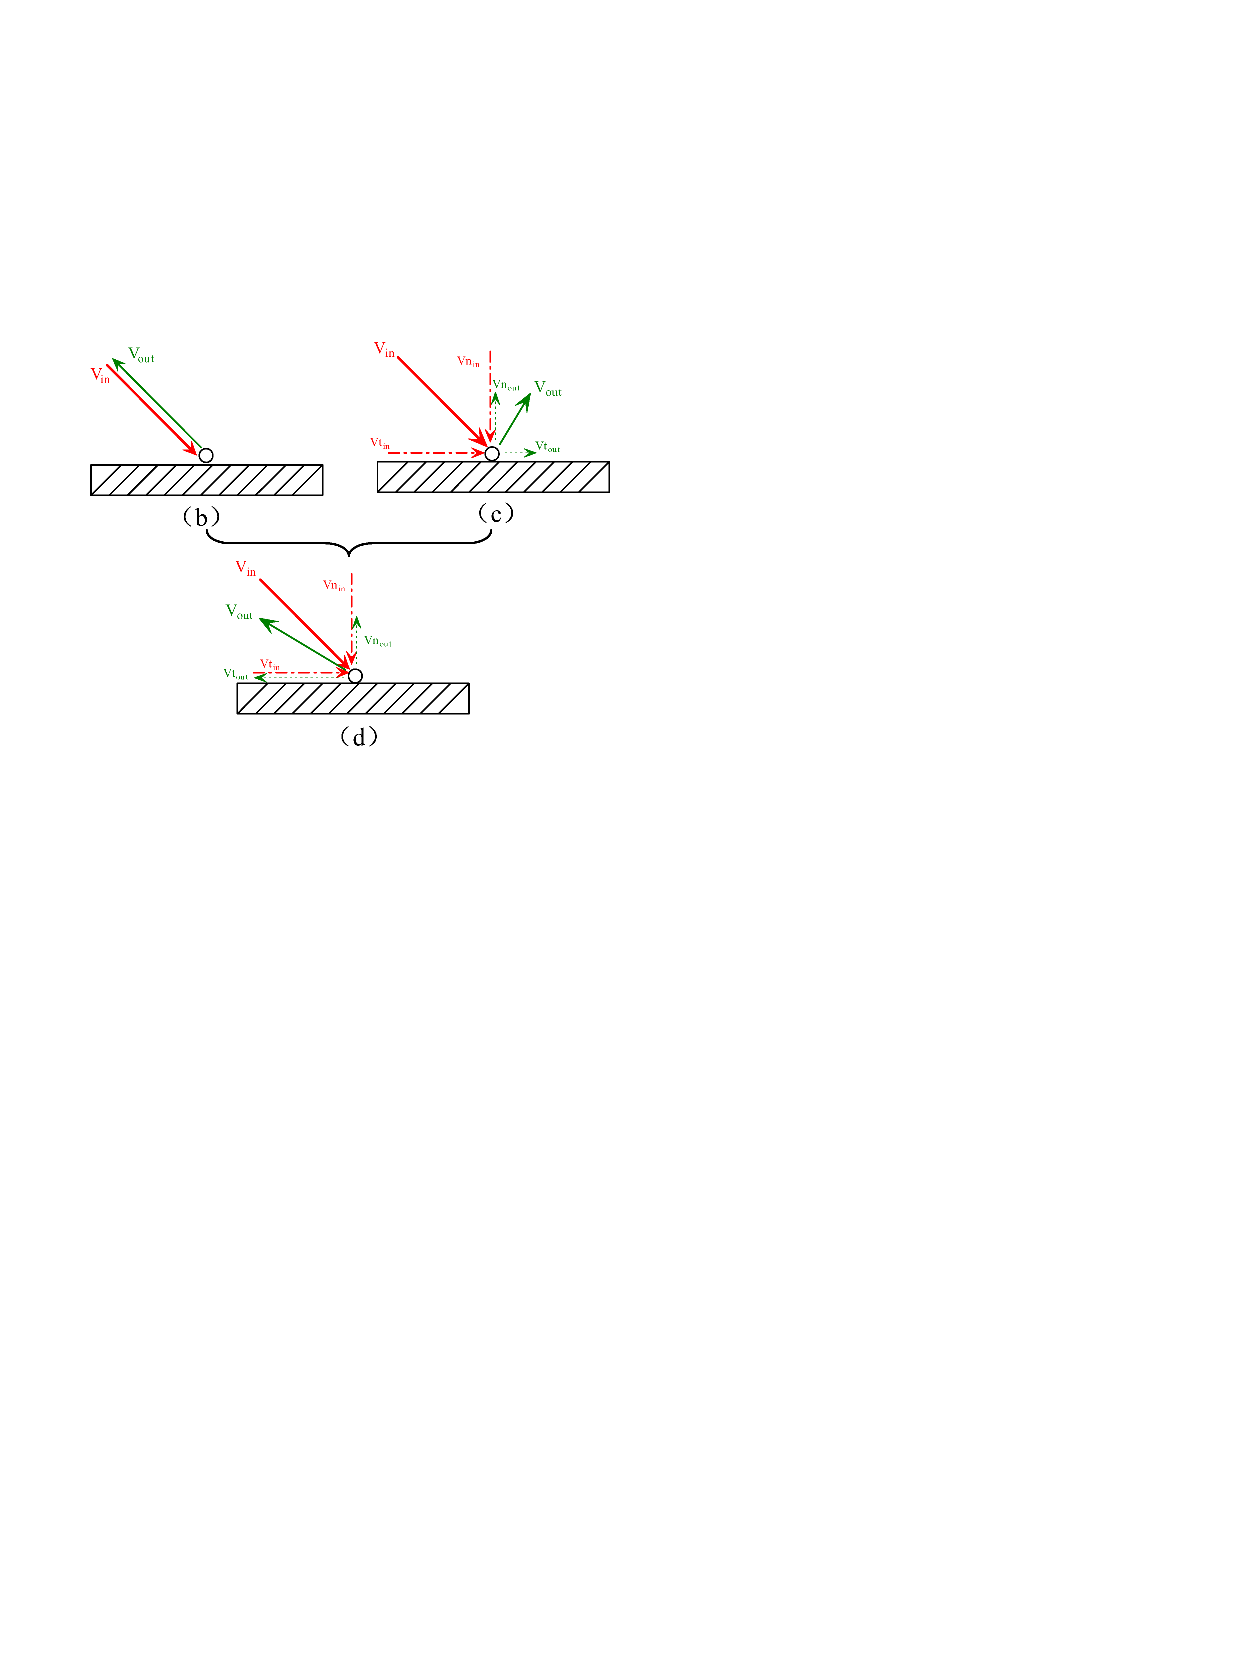
\includegraphics[width=1\textwidth]{./figures/fig06.pdf}
\end{column}
\begin{column}[c]{0.5\textwidth}
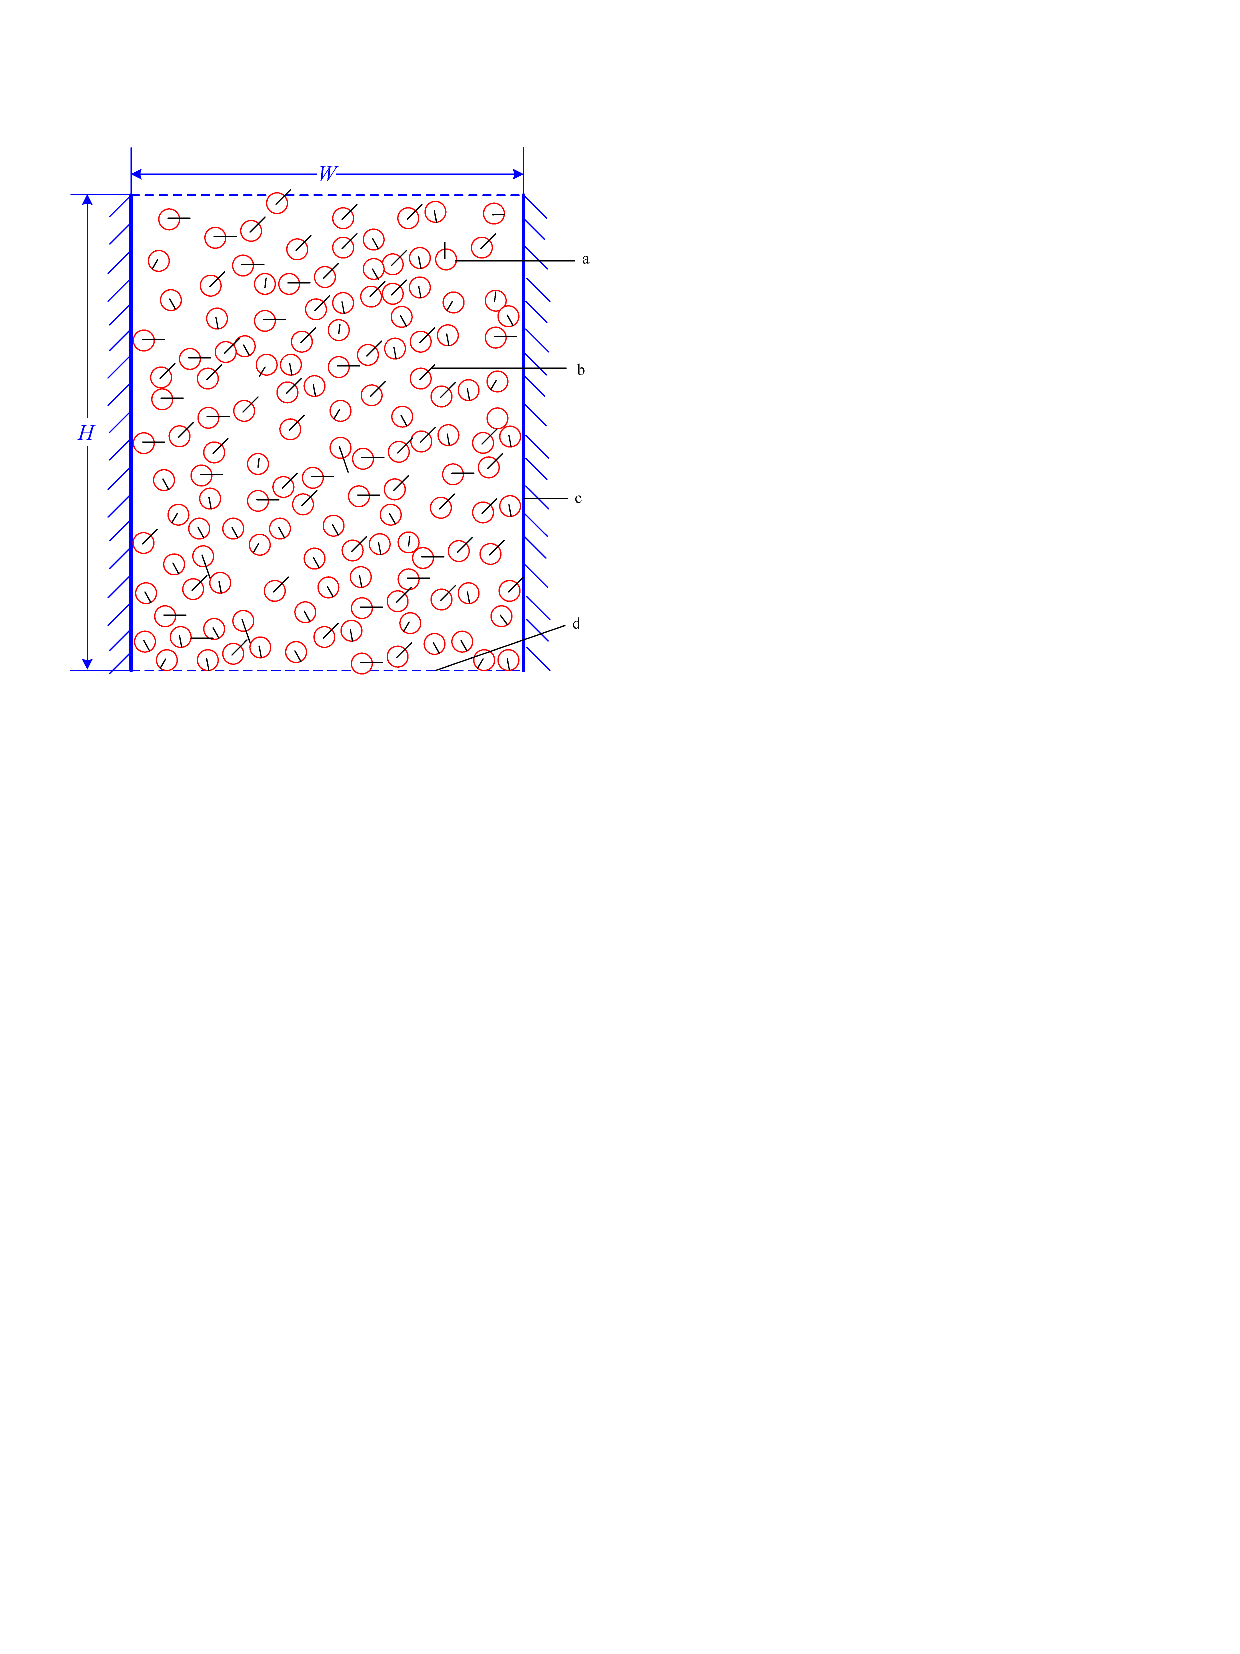
\includegraphics[width=1\textwidth]{./figures/fig07.pdf}
\end{column}
\end{columns}
}

\frame{\frametitle{模型}
与边界作用前后速度分别为
\[
V = v_n\mathbf{n}+v_t\mathbf{\tau}
,
V' = -[(1-\alpha)v_n+\alpha u]\mathbf{n}-v_t\mathbf{\tau}
\]
其中$u$服从
\[
F(u)=2\beta^2u\exp(-\beta^2u^2)
,
 \beta = (2k_b/mT_w)^{-1/2}
\]

Pseudo-particle modeling(PPM): 粒子与粒子作用前后速度$v_1$,$v_{10}$
\[
v_1 = v_{10}-\frac{2m_2}{m_1+m_2}\cdot\frac{(v_{10}-v_{20})\cdot(P_1-P_2)}{|P_1-P2|^2}(P_1-P_2)
\]

}

\subsection{结果}
\frame{\frametitle{两边界的温度相等的结果}
\begin{columns}
\begin{column}[c]{0.5\textwidth}
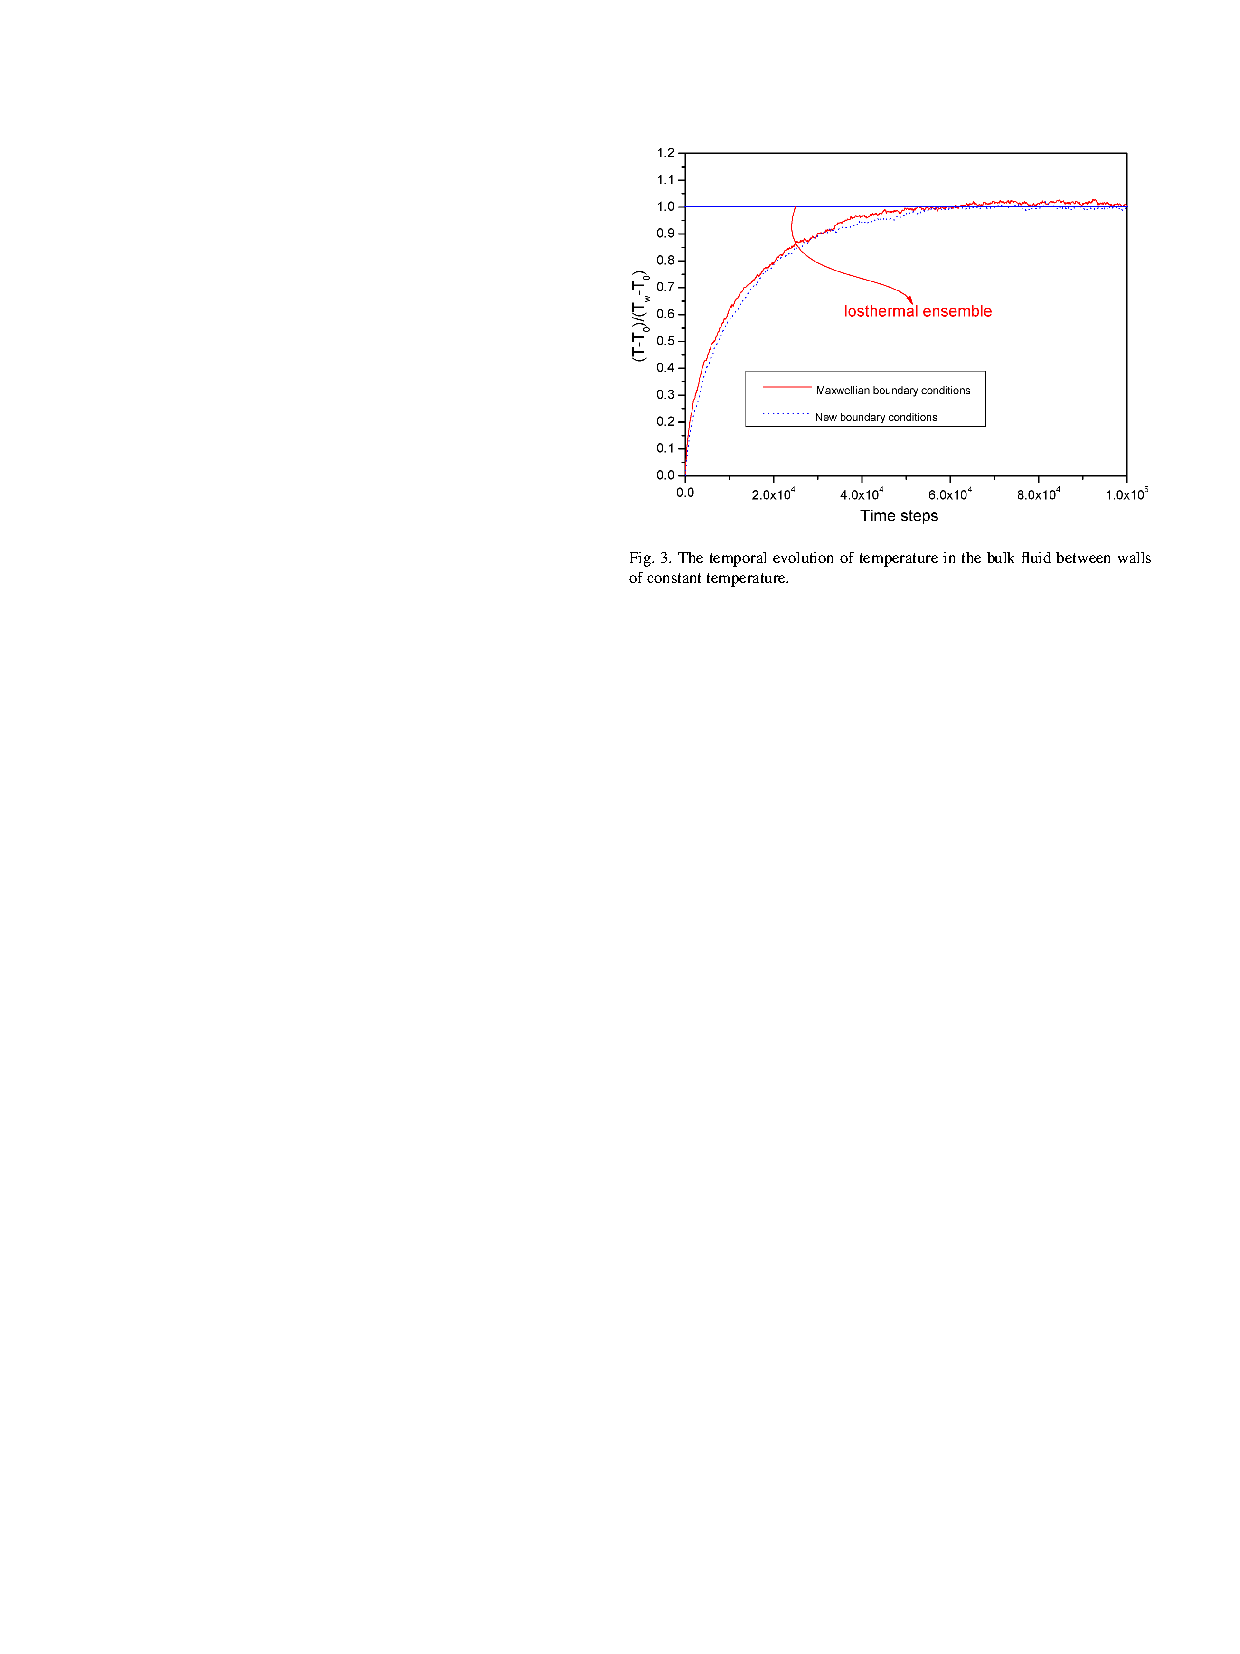
\includegraphics[width=1\textwidth]{./figures/fig08.pdf}
\end{column}
\begin{column}[c]{0.5\textwidth}
两边界的温度相等
\[
T_1=\frac{mv_1^2}{2k_b}=T_2=\frac{mv_2^2}{2k_b}>T_0
\]
\end{column}
\end{columns}
}


\frame{\frametitle{两边界的温度不等的结果}
\begin{columns}
\begin{column}[c]{0.5\textwidth}
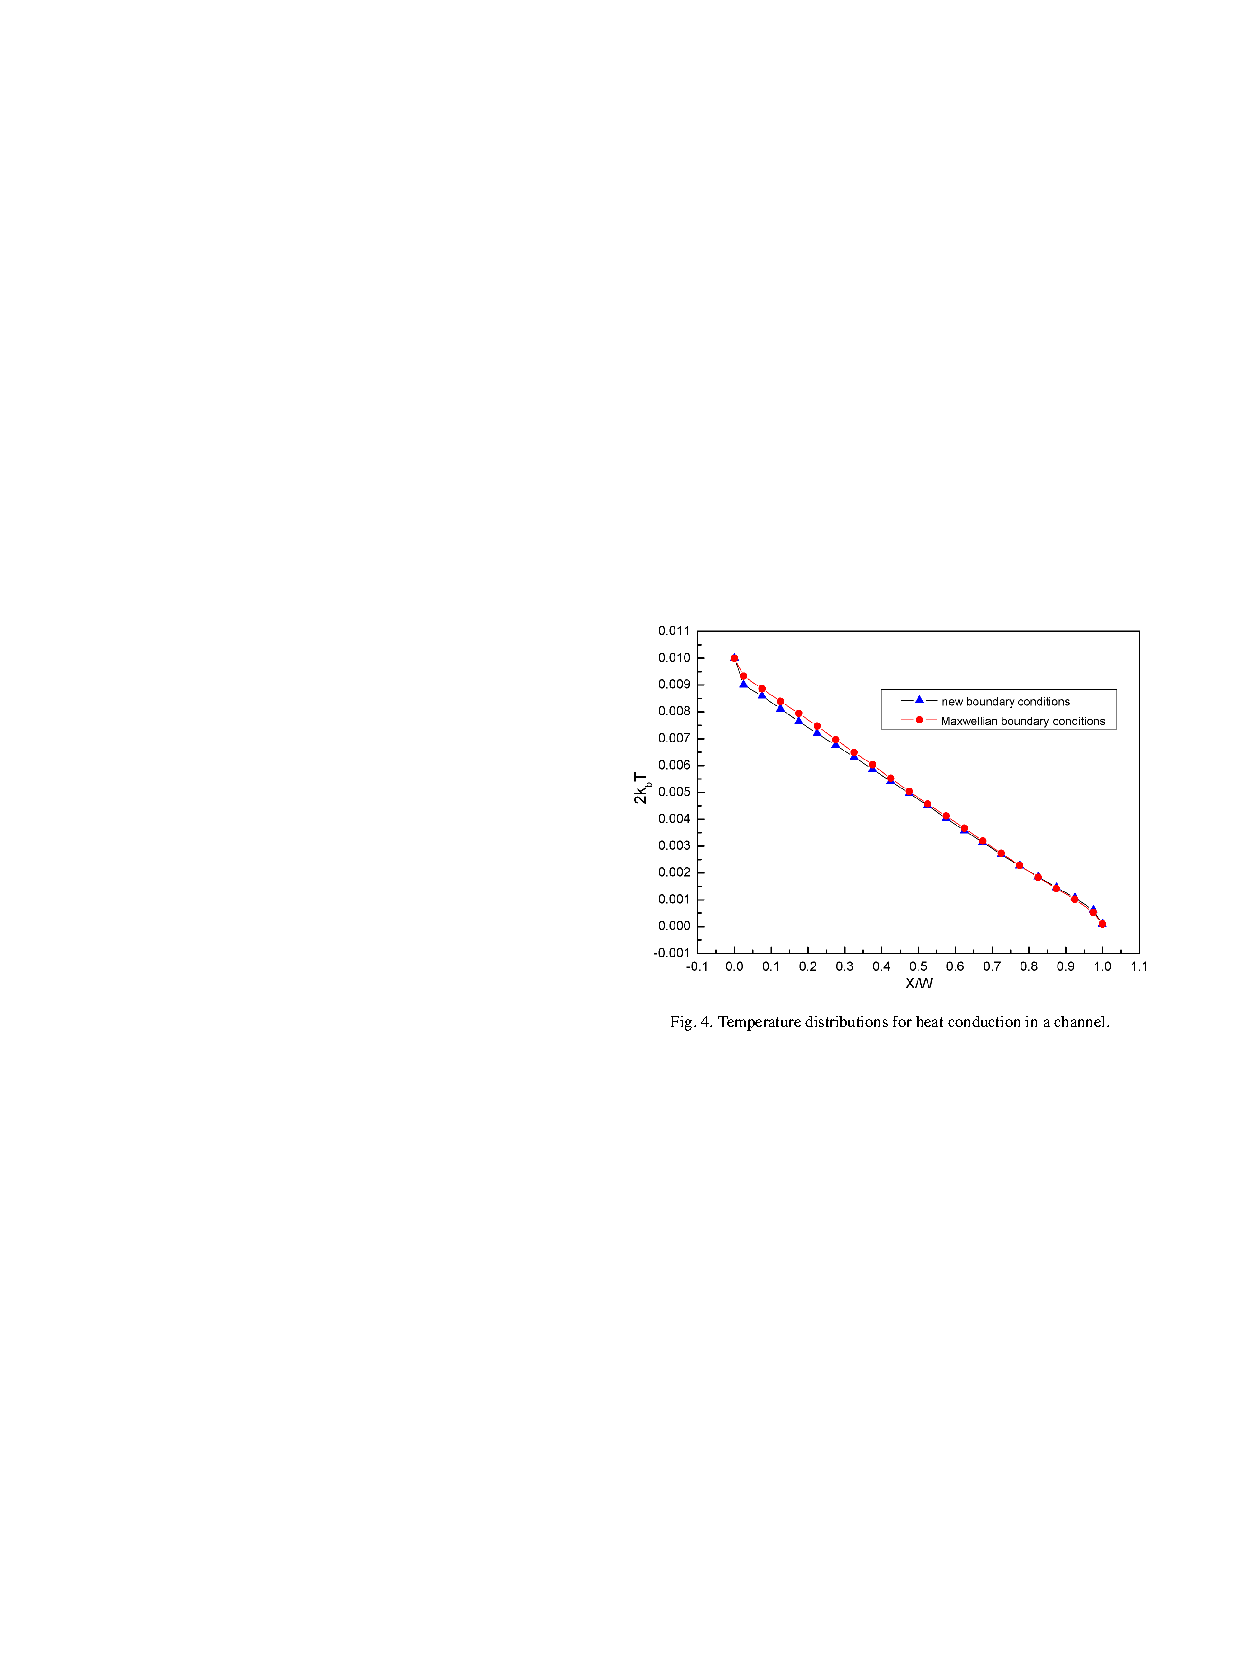
\includegraphics[width=1\textwidth]{./figures/fig09.pdf}
\end{column}
\begin{column}[c]{0.5\textwidth}
两边界的温度不等
\[
T_1=\frac{mv_1^2}{2k_b}>T_0>T_2=\frac{mv_2^2}{2k_b}
\]
\end{column}
\end{columns}
}

\frame{\frametitle{加重力场的结果}
\begin{center}
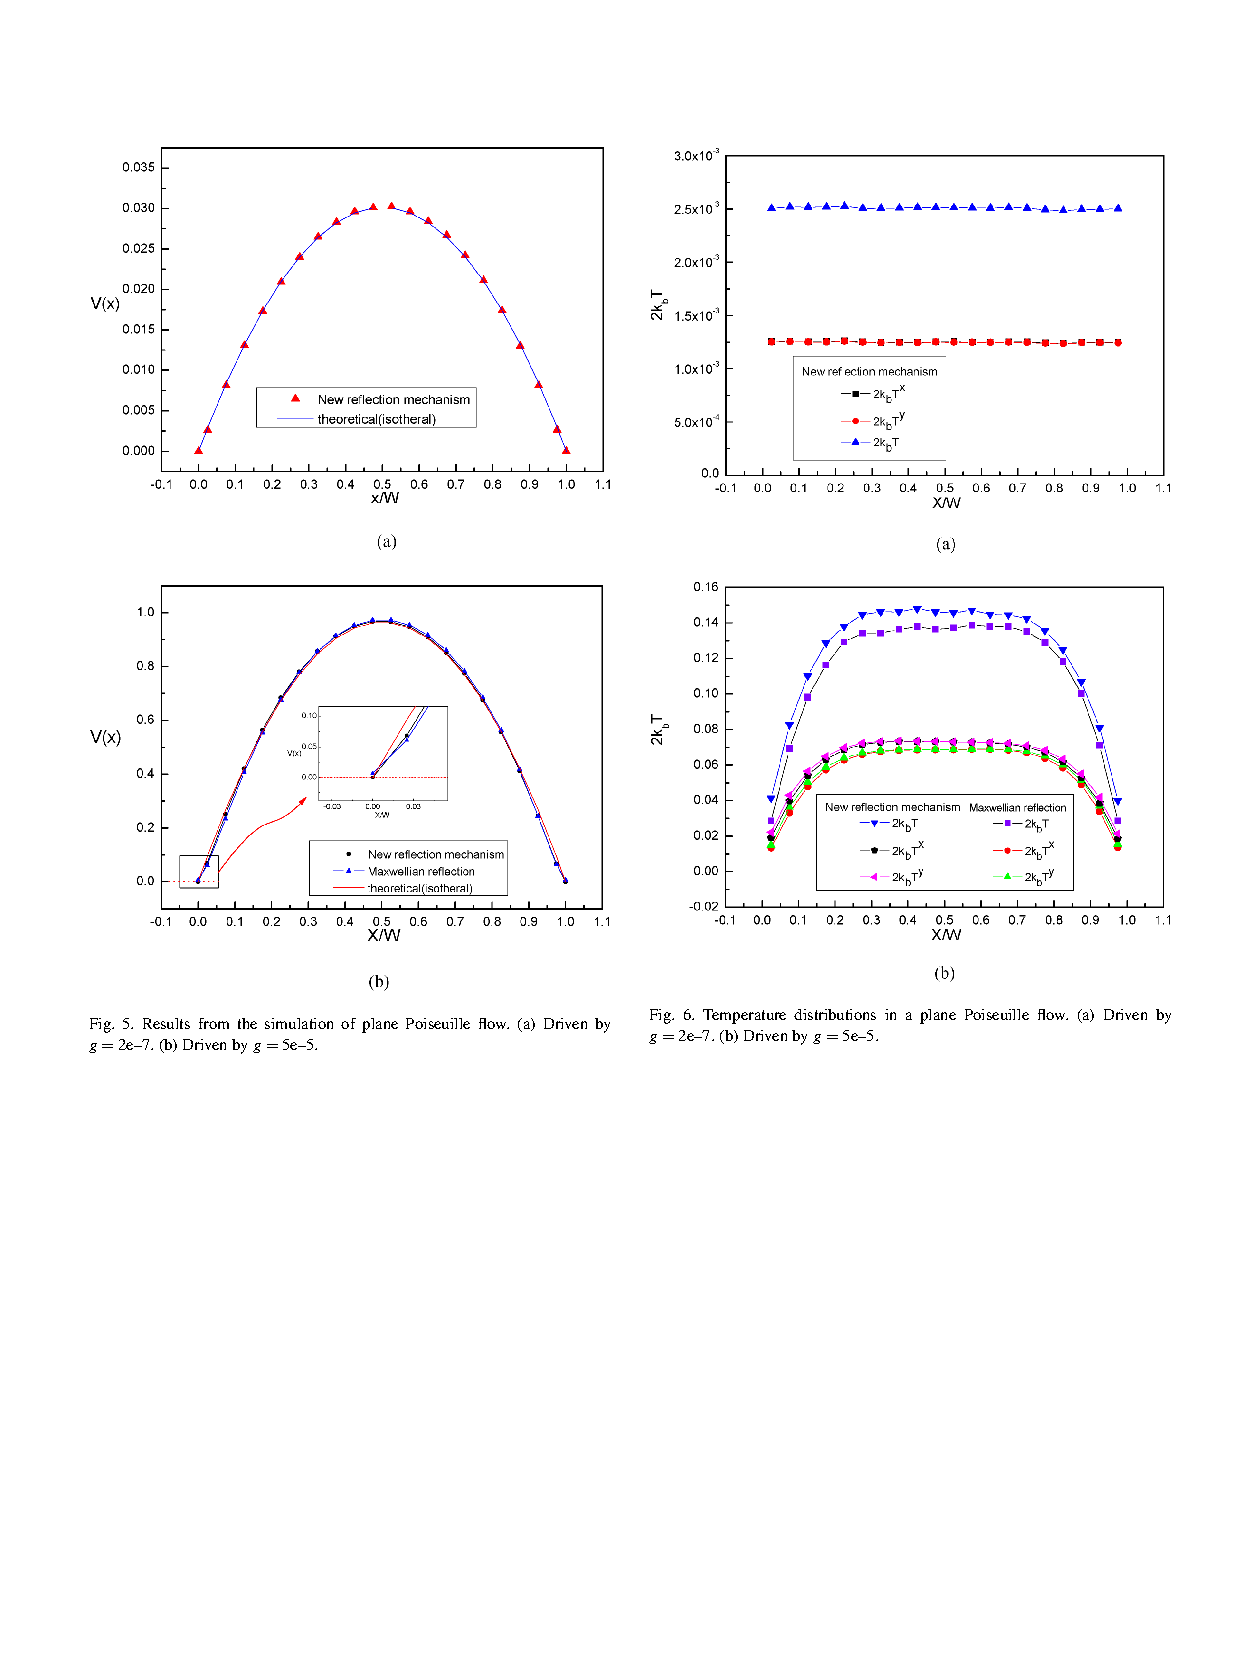
\includegraphics[width=0.77\textwidth]{./figures/fig10.pdf}
\end{center}
}
